% -*- mode: latex; mode: flyspell; ispell-local-dictionary: "en_US"; coding: utf-8; fill-column: 80 -*-

\documentclass{article}

\usepackage[utf8]{inputenc}
\usepackage[english]{babel}

\usepackage{amsmath,amsfonts,amssymb}
\usepackage{fullpage}
\usepackage{verbatim}

\usepackage{tikz,pgfplots}

\pgfplotsset{
  width=150mm,height=100mm,
  major grid style={thin,dotted,color=black!50},
  minor grid style={thin,dotted,color=black!50},
  grid,
  every axis/.append style={
    line width=0.5pt,
    tick style={
      line cap=round,
      thin,
      major tick length=4pt,
      minor tick length=2pt,
    },
  },
  legend cell align=left,
  legend pos=north west,
}

%%%%%%%%%%%%%%%%%%%%%%%%%%%%%%%%%%%%%%%%%%%%%%%%%%%%%%%%%%%%%%%%%%%%%%%%%%%%%%%%

\begin{document}

\title{Prezza LCE Tests}
\author{Alexander Herlez}
\maketitle

%IMPORT-DATA stats time.txt

\begin{center}
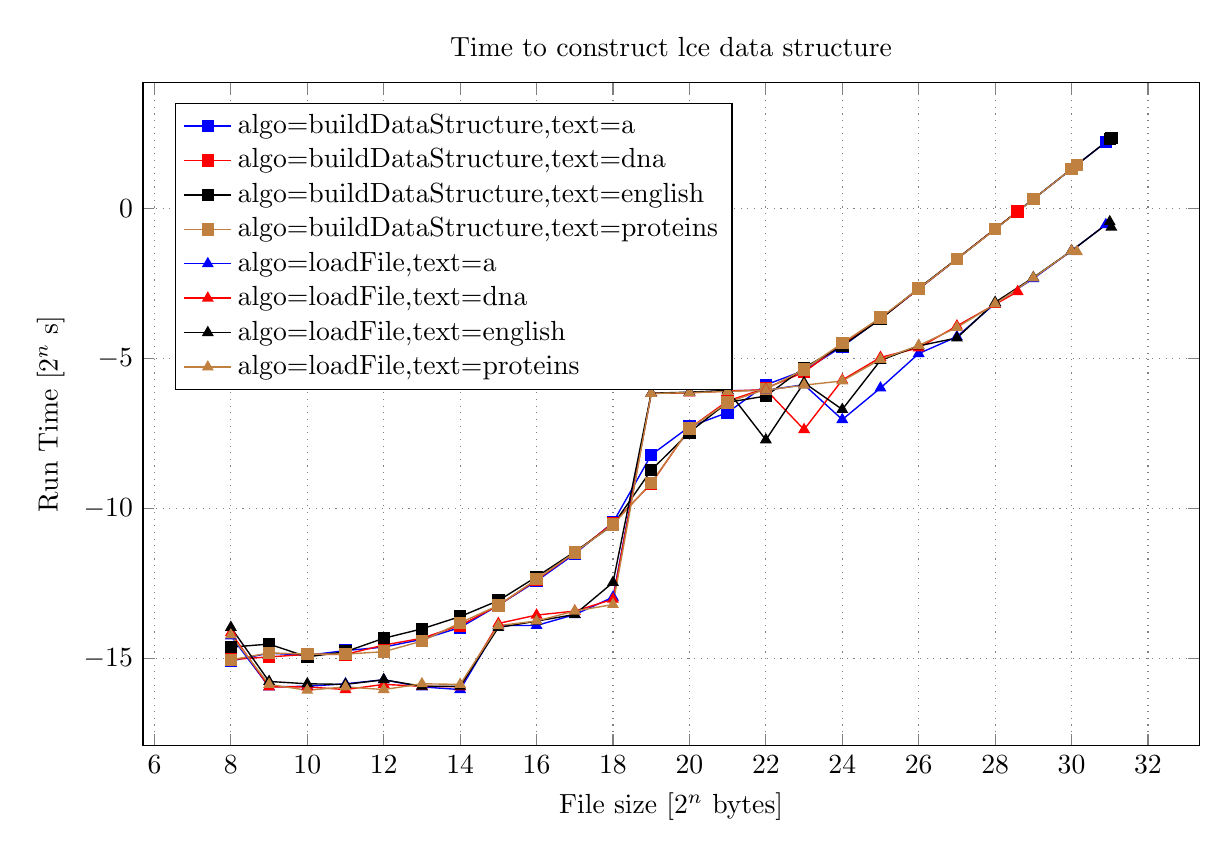
\begin{tikzpicture}
  \begin{axis}[
    title={Time to construct lce data structure},
    xlabel={File size [$2^n$ bytes]},
    ylabel={Run Time [$2^n$ s]},
    ]

    %% MULTIPLOT(algo, text) SELECT LOG(2, size) AS x, LOG(2, time) AS y, MULTIPLOT
    %% FROM stats WHERE algo = "loadFile" OR algo = "buildDataStructure" GROUP BY MULTIPLOT,x  ORDER BY MULTIPLOT,x
    \addplot[blue, mark=square*] coordinates { (8.0,-15.0693) (9.0,-14.8102) (10.0,-14.8811) (11.0,-14.7239) (12.0,-14.6077) (13.0,-14.3489) (14.0,-13.9556) (15.0,-13.2154) (16.0,-12.4075) (17.0,-11.5011) (18.0,-10.4579) (19.0,-8.20579) (20.0,-7.26513) (21.0,-6.79184) (22.0,-5.86885) (23.0,-5.3938) (24.0,-4.59364) (25.0,-3.66476) (26.0,-2.6787) (27.0,-1.68052) (28.0,-0.676861) (29.0,0.317431) (30.0,1.3235) (30.8974,2.21598) };
    \addlegendentry{algo=buildDataStructure,text=a};
    \addplot[red, mark=square*] coordinates { (8.0,-15.0227) (9.0,-14.9339) (10.0,-14.8503) (11.0,-14.8503) (12.0,-14.5406) (13.0,-14.3135) (14.0,-13.8863) (15.0,-13.2186) (16.0,-12.3688) (17.0,-11.4599) (18.0,-10.4804) (19.0,-9.16257) (20.0,-7.32145) (21.0,-6.40728) (22.0,-5.98338) (23.0,-5.44909) (24.0,-4.50911) (25.0,-3.67186) (26.0,-2.67163) (27.0,-1.67642) (28.0,-0.672499) (28.5895,-0.093211) };
    \addlegendentry{algo=buildDataStructure,text=dna};
    \addplot[black, mark=square*] coordinates { (8.0,-14.6077) (9.0,-14.5081) (10.0,-14.9339) (11.0,-14.7616) (12.0,-14.3135) (13.0,-14) (14.0,-13.5906) (15.0,-13.0604) (16.0,-12.2653) (17.0,-11.432) (18.0,-10.5411) (19.0,-8.71359) (20.0,-7.45106) (21.0,-6.45229) (22.0,-6.24407) (23.0,-5.30023) (24.0,-4.57185) (25.0,-3.68075) (26.0,-2.64998) (27.0,-1.67381) (28.0,-0.678003) (29.0,0.320173) (30.0,1.32345) (31.0,2.32258) (31.0417,2.35808) };
    \addlegendentry{algo=buildDataStructure,text=english};
    \addplot[brown, mark=square*] coordinates { (8.0,-15.0342) (9.0,-14.8003) (10.0,-14.8401) (11.0,-14.8401) (12.0,-14.7616) (13.0,-14.4075) (14.0,-13.8003) (15.0,-13.2154) (16.0,-12.3472) (17.0,-11.455) (18.0,-10.5263) (19.0,-9.13949) (20.0,-7.32768) (21.0,-6.45416) (22.0,-6.01464) (23.0,-5.35557) (24.0,-4.48084) (25.0,-3.6337) (26.0,-2.6663) (27.0,-1.68353) (28.0,-0.685742) (29.0,0.31676) (30.0,1.32348) (30.1411,1.45831) };
    \addlegendentry{algo=buildDataStructure,text=proteins};
    \addplot[blue, mark=triangle*] coordinates { (8.0,-14.2318) (9.0,-15.9339) (10.0,-15.9125) (11.0,-15.8301) (12.0,-15.6962) (13.0,-15.9339) (14.0,-16.0227) (15.0,-13.8915) (16.0,-13.8863) (17.0,-13.5243) (18.0,-12.9447) (19.0,-6.15505) (20.0,-6.12682) (21.0,-6.06438) (22.0,-6.0514) (23.0,-5.86365) (24.0,-7.02805) (25.0,-5.9762) (26.0,-4.82853) (27.0,-4.26782) (28.0,-3.15851) (29.0,-2.32922) (30.0,-1.40386) (30.8974,-0.533034) };
    \addlegendentry{algo=loadFile,text=a};
    \addplot[red, mark=triangle*] coordinates { (8.0,-14.1235) (9.0,-15.9339) (10.0,-15.9339) (11.0,-16.0227) (12.0,-15.8503) (13.0,-15.9125) (14.0,-15.9339) (15.0,-13.8201) (16.0,-13.5406) (17.0,-13.4075) (18.0,-13.0142) (19.0,-6.15647) (20.0,-6.13775) (21.0,-6.07542) (22.0,-6.03232) (23.0,-7.35959) (24.0,-5.70946) (25.0,-4.95689) (26.0,-4.63806) (27.0,-3.90736) (28.0,-3.19088) (28.5895,-2.76202) };
    \addlegendentry{algo=loadFile,text=dna};
    \addplot[black, mark=triangle*] coordinates { (8.0,-13.9502) (9.0,-15.7521) (10.0,-15.8301) (11.0,-15.8503) (12.0,-15.6962) (13.0,-15.9125) (14.0,-15.9125) (15.0,-13.9556) (16.0,-13.7426) (17.0,-13.5202) (18.0,-12.455) (19.0,-6.14786) (20.0,-6.11449) (21.0,-6.05572) (22.0,-7.70273) (23.0,-5.79835) (24.0,-6.69035) (25.0,-5.0538) (26.0,-4.56996) (27.0,-4.30866) (28.0,-3.12166) (29.0,-2.2936) (30.0,-1.40465) (31.0,-0.436951) (31.0417,-0.617375) };
    \addlegendentry{algo=loadFile,text=english};
    \addplot[brown, mark=triangle*] coordinates { (8.0,-14.2056) (9.0,-15.8503) (10.0,-16.0458) (11.0,-15.9339) (12.0,-16.0227) (13.0,-15.8301) (14.0,-15.8503) (15.0,-13.8915) (16.0,-13.7379) (17.0,-13.4075) (18.0,-13.1894) (19.0,-6.15729) (20.0,-6.13026) (21.0,-6.09051) (22.0,-6.04883) (23.0,-5.87918) (24.0,-5.74134) (25.0,-5.02074) (26.0,-4.5602) (27.0,-3.96025) (28.0,-3.17685) (29.0,-2.30728) (30.0,-1.40473) (30.1411,-1.4323) };
    \addlegendentry{algo=loadFile,text=proteins};
    

  \end{axis}
\end{tikzpicture}
\end{center}

\begin{center}
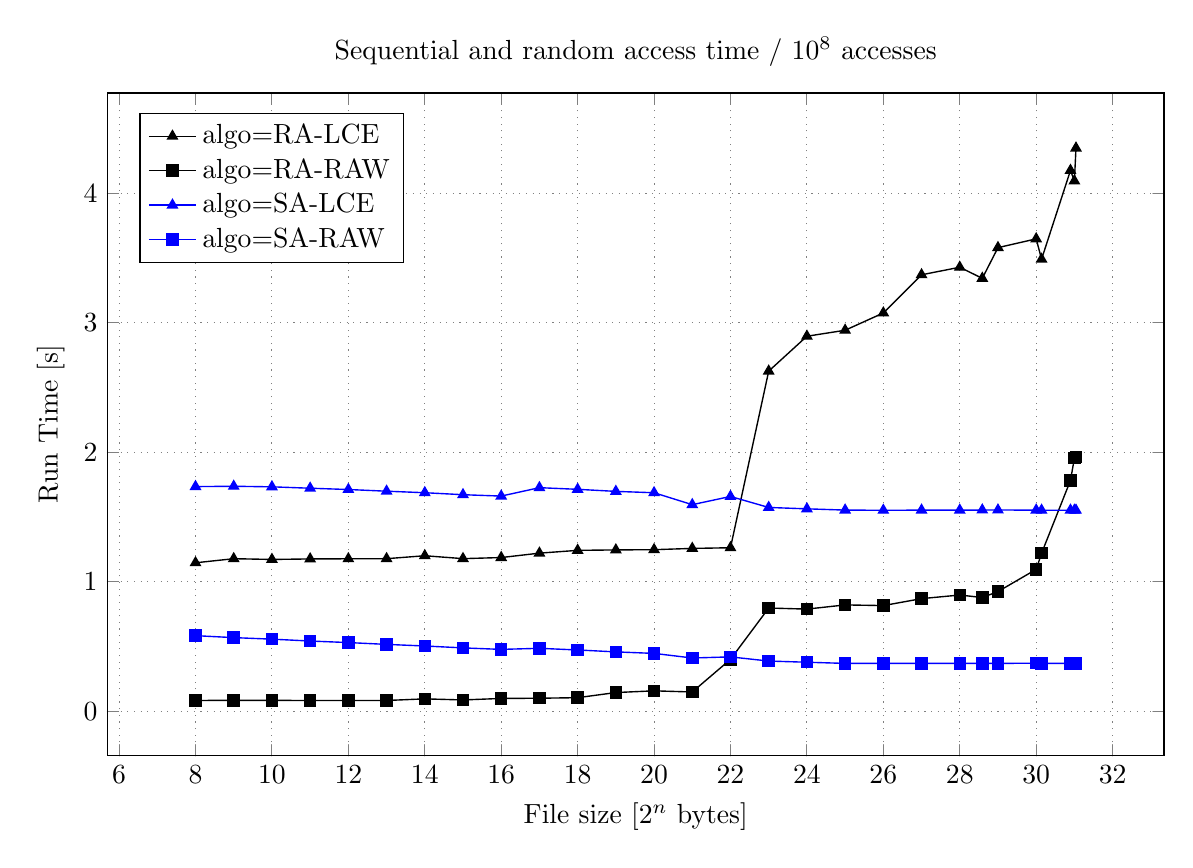
\begin{tikzpicture}
  \begin{axis}[
    title={Sequential and random access time / $10^8$ accesses},
    xlabel={File size [$2^n$ bytes]},
    ylabel={Run Time [s]},
    ]

    %% MULTIPLOT(algo) SELECT LOG(2, size) AS x, time AS y, MULTIPLOT
    %% FROM stats WHERE algo = "RA-LCE" OR algo = "RA-RAW" OR algo = "SA-LCE" OR algo = "SA-RAW" GROUP BY MULTIPLOT,x  ORDER BY MULTIPLOT,x
    \addplot[black, mark=triangle*] coordinates { (8.0,1.14657) (9.0,1.17813) (10.0,1.17236) (11.0,1.17629) (12.0,1.17754) (13.0,1.17828) (14.0,1.20101) (15.0,1.17863) (16.0,1.187) (17.0,1.22102) (18.0,1.24259) (19.0,1.24594) (20.0,1.24784) (21.0,1.25759) (22.0,1.26268) (23.0,2.6266) (24.0,2.89596) (25.0,2.9422) (26.0,3.0756) (27.0,3.37051) (28.0,3.42868) (28.5895,3.3431) (29.0,3.58015) (30.0,3.64795) (30.1411,3.49096) (30.8974,4.17626) (31.0,4.09523) (31.0417,4.34881) };
    \addlegendentry{algo=RA-LCE};
    \addplot[black, mark=square*] coordinates { (8.0,0.083472) (9.0,0.0838721) (10.0,0.0836961) (11.0,0.0835102) (12.0,0.083195) (13.0,0.0833151) (14.0,0.0957391) (15.0,0.087491) (16.0,0.098995) (17.0,0.10072) (18.0,0.104895) (19.0,0.144523) (20.0,0.157777) (21.0,0.148905) (22.0,0.400892) (23.0,0.797178) (24.0,0.788955) (25.0,0.821205) (26.0,0.816149) (27.0,0.869757) (28.0,0.897607) (28.5895,0.87826) (29.0,0.924342) (30.0,1.09563) (30.1411,1.22033) (30.8974,1.78271) (31.0,1.95372) (31.0417,1.9617) };
    \addlegendentry{algo=RA-RAW};
    \addplot[blue, mark=triangle*] coordinates { (8.0,1.73481) (9.0,1.73746) (10.0,1.73316) (11.0,1.72232) (12.0,1.71242) (13.0,1.69935) (14.0,1.68767) (15.0,1.6723) (16.0,1.66164) (17.0,1.72662) (18.0,1.71387) (19.0,1.69794) (20.0,1.68745) (21.0,1.59538) (22.0,1.6588) (23.0,1.57377) (24.0,1.56321) (25.0,1.55351) (26.0,1.55203) (27.0,1.55317) (28.0,1.55297) (28.5895,1.55391) (29.0,1.55394) (30.0,1.55348) (30.1411,1.55223) (30.8974,1.55271) (31.0,1.55222) (31.0417,1.55218) };
    \addlegendentry{algo=SA-LCE};
    \addplot[blue, mark=square*] coordinates { (8.0,0.583882) (9.0,0.568652) (10.0,0.556904) (11.0,0.542374) (12.0,0.530496) (13.0,0.516417) (14.0,0.504089) (15.0,0.489413) (16.0,0.477855) (17.0,0.486076) (18.0,0.473332) (19.0,0.458521) (20.0,0.446859) (21.0,0.411401) (22.0,0.419922) (23.0,0.387762) (24.0,0.378616) (25.0,0.369645) (26.0,0.369411) (27.0,0.369977) (28.0,0.36972) (28.5895,0.369743) (29.0,0.369721) (30.0,0.371223) (30.1411,0.369433) (30.8974,0.369507) (31.0,0.369462) (31.0417,0.36939) };
    \addlegendentry{algo=SA-RAW};
  \end{axis}
\end{tikzpicture}
\end{center}



\begin{center}
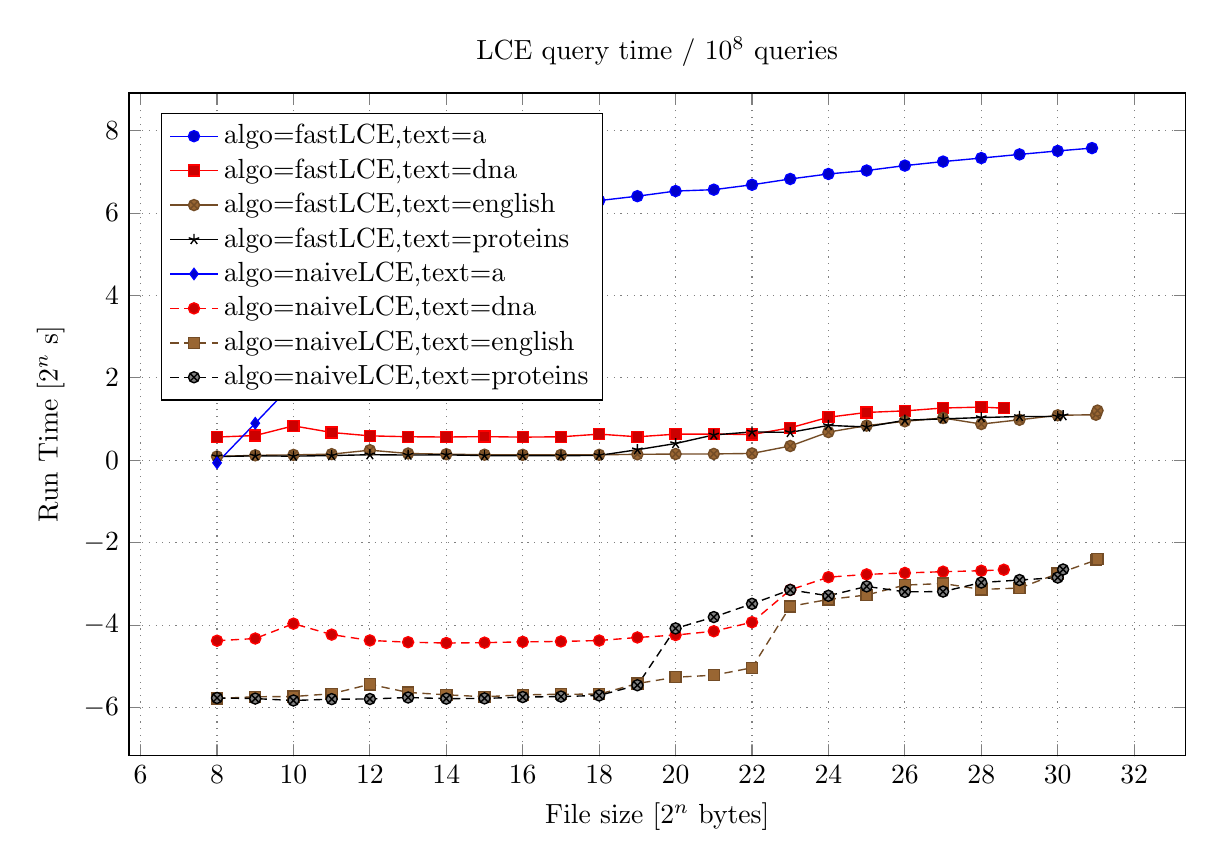
\begin{tikzpicture}
  \begin{axis}[
    title={LCE query time / $10^8$ queries},
    xlabel={File size [$2^n$ bytes]},
    ylabel={Run Time [$2^n$ s]},
    ]

    %% MULTIPLOT(algo, text) SELECT LOG(2, size) AS x, LOG(2, time) AS y, MULTIPLOT
    %% FROM stats WHERE algo = "fastLCE" OR algo = "naiveLCE" GROUP BY MULTIPLOT,x  ORDER BY MULTIPLOT,x
    \addplot coordinates { (8.0,4.45942) (9.0,4.76717) (10.0,4.98458) (11.0,5.2001) (12.0,5.39791) (13.0,5.57759) (14.0,5.74506) (15.0,5.86234) (16.0,6.00496) (17.0,6.2276) (18.0,6.30285) (19.0,6.40991) (20.0,6.53399) (21.0,6.56774) (22.0,6.68665) (23.0,6.8272) (24.0,6.9491) (25.0,7.03235) (26.0,7.15163) (27.0,7.24951) (28.0,7.33495) (29.0,7.4234) (30.0,7.50787) (30.8974,7.57653) };
    \addlegendentry{algo=fastLCE,text=a};
    \addplot coordinates { (8.0,0.565344) (9.0,0.602371) (10.0,0.837201) (11.0,0.67634) (12.0,0.594577) (13.0,0.573122) (14.0,0.566055) (15.0,0.576135) (16.0,0.563412) (17.0,0.57189) (18.0,0.636154) (19.0,0.571881) (20.0,0.635467) (21.0,0.637332) (22.0,0.626962) (23.0,0.789253) (24.0,1.04586) (25.0,1.16311) (26.0,1.20071) (27.0,1.27012) (28.0,1.29242) (28.5895,1.26582) };
    \addlegendentry{algo=fastLCE,text=dna};
    \addplot coordinates { (8.0,0.0938846) (9.0,0.122341) (10.0,0.133182) (11.0,0.150924) (12.0,0.247271) (13.0,0.16678) (14.0,0.149624) (15.0,0.137543) (16.0,0.134996) (17.0,0.133537) (18.0,0.135154) (19.0,0.146134) (20.0,0.153455) (21.0,0.15606) (22.0,0.167705) (23.0,0.347904) (24.0,0.685824) (25.0,0.843349) (26.0,0.948063) (27.0,1.02807) (28.0,0.880858) (29.0,0.98429) (30.0,1.09371) (31.0,1.10697) (31.0417,1.20819) };
    \addlegendentry{algo=fastLCE,text=english};
    \addplot coordinates { (8.0,0.0921668) (9.0,0.109548) (10.0,0.101932) (11.0,0.11687) (12.0,0.13669) (13.0,0.129204) (14.0,0.133537) (15.0,0.115952) (16.0,0.116045) (17.0,0.11234) (18.0,0.120498) (19.0,0.258012) (20.0,0.408201) (21.0,0.617233) (22.0,0.690623) (23.0,0.678577) (24.0,0.847412) (25.0,0.811422) (26.0,0.973031) (27.0,1.00711) (28.0,1.03768) (29.0,1.06402) (30.0,1.0627) (30.1411,1.0844) };
    \addlegendentry{algo=fastLCE,text=proteins};
    \addplot coordinates { (8.0,-0.0605838) (9.0,0.901579) (10.0,1.87255) (11.0,2.86111) (12.0,3.85657) (13.0,4.85287) };
    \addlegendentry{algo=naiveLCE,text=a};
    \addplot coordinates { (8.0,-4.37614) (9.0,-4.32273) (10.0,-3.9624) (11.0,-4.22772) (12.0,-4.36929) (13.0,-4.41166) (14.0,-4.43203) (15.0,-4.42309) (16.0,-4.40372) (17.0,-4.39362) (18.0,-4.37157) (19.0,-4.29741) (20.0,-4.23917) (21.0,-4.14581) (22.0,-3.92768) (23.0,-3.14261) (24.0,-2.8338) (25.0,-2.76655) (26.0,-2.73195) (27.0,-2.70126) (28.0,-2.67829) (28.5895,-2.65391) };
    \addlegendentry{algo=naiveLCE,text=dna};
    \addplot coordinates { (8.0,-5.77896) (9.0,-5.73581) (10.0,-5.73) (11.0,-5.66295) (12.0,-5.43422) (13.0,-5.63066) (14.0,-5.68832) (15.0,-5.73605) (16.0,-5.69047) (17.0,-5.67448) (18.0,-5.67255) (19.0,-5.4142) (20.0,-5.26224) (21.0,-5.21293) (22.0,-5.03245) (23.0,-3.54313) (24.0,-3.37442) (25.0,-3.2667) (26.0,-3.02666) (27.0,-2.98799) (28.0,-3.13169) (29.0,-3.09785) (30.0,-2.74916) (31.0,-2.42073) (31.0417,-2.39464) };
    \addlegendentry{algo=naiveLCE,text=english};
    \addplot coordinates { (8.0,-5.76509) (9.0,-5.78015) (10.0,-5.82656) (11.0,-5.79362) (12.0,-5.79059) (13.0,-5.75369) (14.0,-5.78144) (15.0,-5.77586) (16.0,-5.74337) (17.0,-5.73089) (18.0,-5.70404) (19.0,-5.45639) (20.0,-4.07709) (21.0,-3.80208) (22.0,-3.48026) (23.0,-3.14355) (24.0,-3.28529) (25.0,-3.05848) (26.0,-3.19005) (27.0,-3.18424) (28.0,-2.9647) (29.0,-2.9035) (30.0,-2.84383) (30.1411,-2.64787) };
    \addlegendentry{algo=naiveLCE,text=proteins};

  \end{axis}
\end{tikzpicture}
\end{center}



%Hallo IMPORT-DATA statsSSS sss.txt


\begin{center}
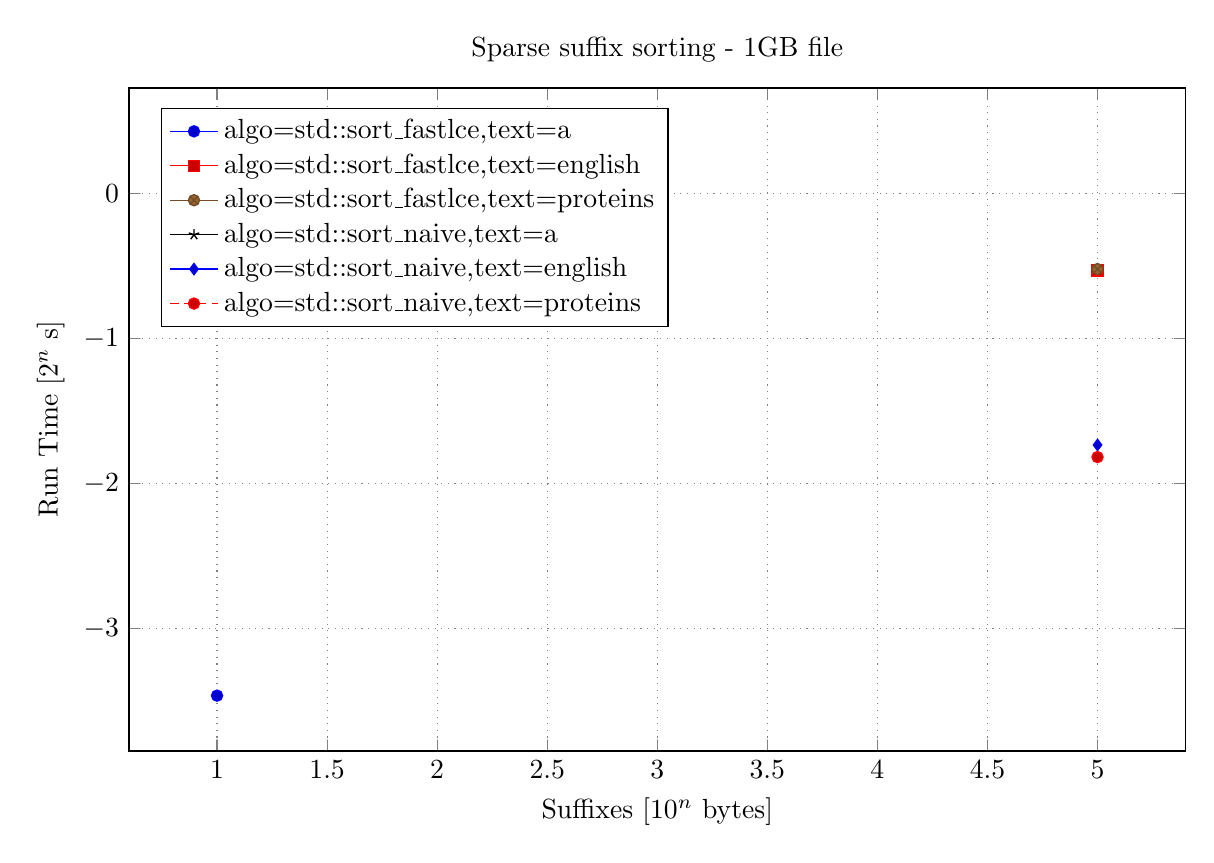
\begin{tikzpicture}
  \begin{axis}[
    title={Sparse suffix sorting - 1GB file},
    xlabel={Suffixes [$10^n$ bytes]},
    ylabel={Run Time [$2^n$ s]},
    ]

    %%% Hallo MULTIPLOT(algo, text) SELECT LOG(2, suffixes) AS x, LOG(2, time) AS y, MULTIPLOT
    %%% FROM stats WHERE algo = "std::sort_naive" OR algo = "std::sort_fastlce" GROUP BY MULTIPLOT,x  ORDER BY MULTIPLOT,x
    \addplot coordinates { (1.0,-3.46219) };
    \addlegendentry{algo=std::sort\_fastlce,text=a};
    \addplot coordinates { (5.0,-0.531991) };
    \addlegendentry{algo=std::sort\_fastlce,text=english};
    \addplot coordinates { (5.0,-0.522727) };
    \addlegendentry{algo=std::sort\_fastlce,text=proteins};
    \addplot coordinates { (1.0,0.344337) };
    \addlegendentry{algo=std::sort\_naive,text=a};
    \addplot coordinates { (5.0,-1.73457) };
    \addlegendentry{algo=std::sort\_naive,text=english};
    \addplot coordinates { (5.0,-1.81827) };
    \addlegendentry{algo=std::sort\_naive,text=proteins};
  \end{axis}
\end{tikzpicture}
\end{center}




\begin{comment}
% TEXTTABLE SELECT COUNT(*), SUM(time) FROM stats
+----------+----------------+
| COUNT(*) |      SUM(time) |
+----------+----------------+
|      742 | 2923.114936234 |
+----------+----------------+
% END TEXTTABLE SELECT COUNT(*), SUM(time) FROM stats
\end{comment}

\end{document}

%%%%%%%%%%%%%%%%%%%%%%%%%%%%%%%%%%%%%%%%%%%%%%%%%%%%%%%%%%%%%%%%%%%%%%%%%%%%%%%%
